\subsection{Per-Task Performance Analysis}
\label{sec:per_task_breakdown}

We analyze performance at the individual task level to identify capability gaps and model-specific trends across all 14 evaluated models.

\begin{figure*}[htbp]
\centering
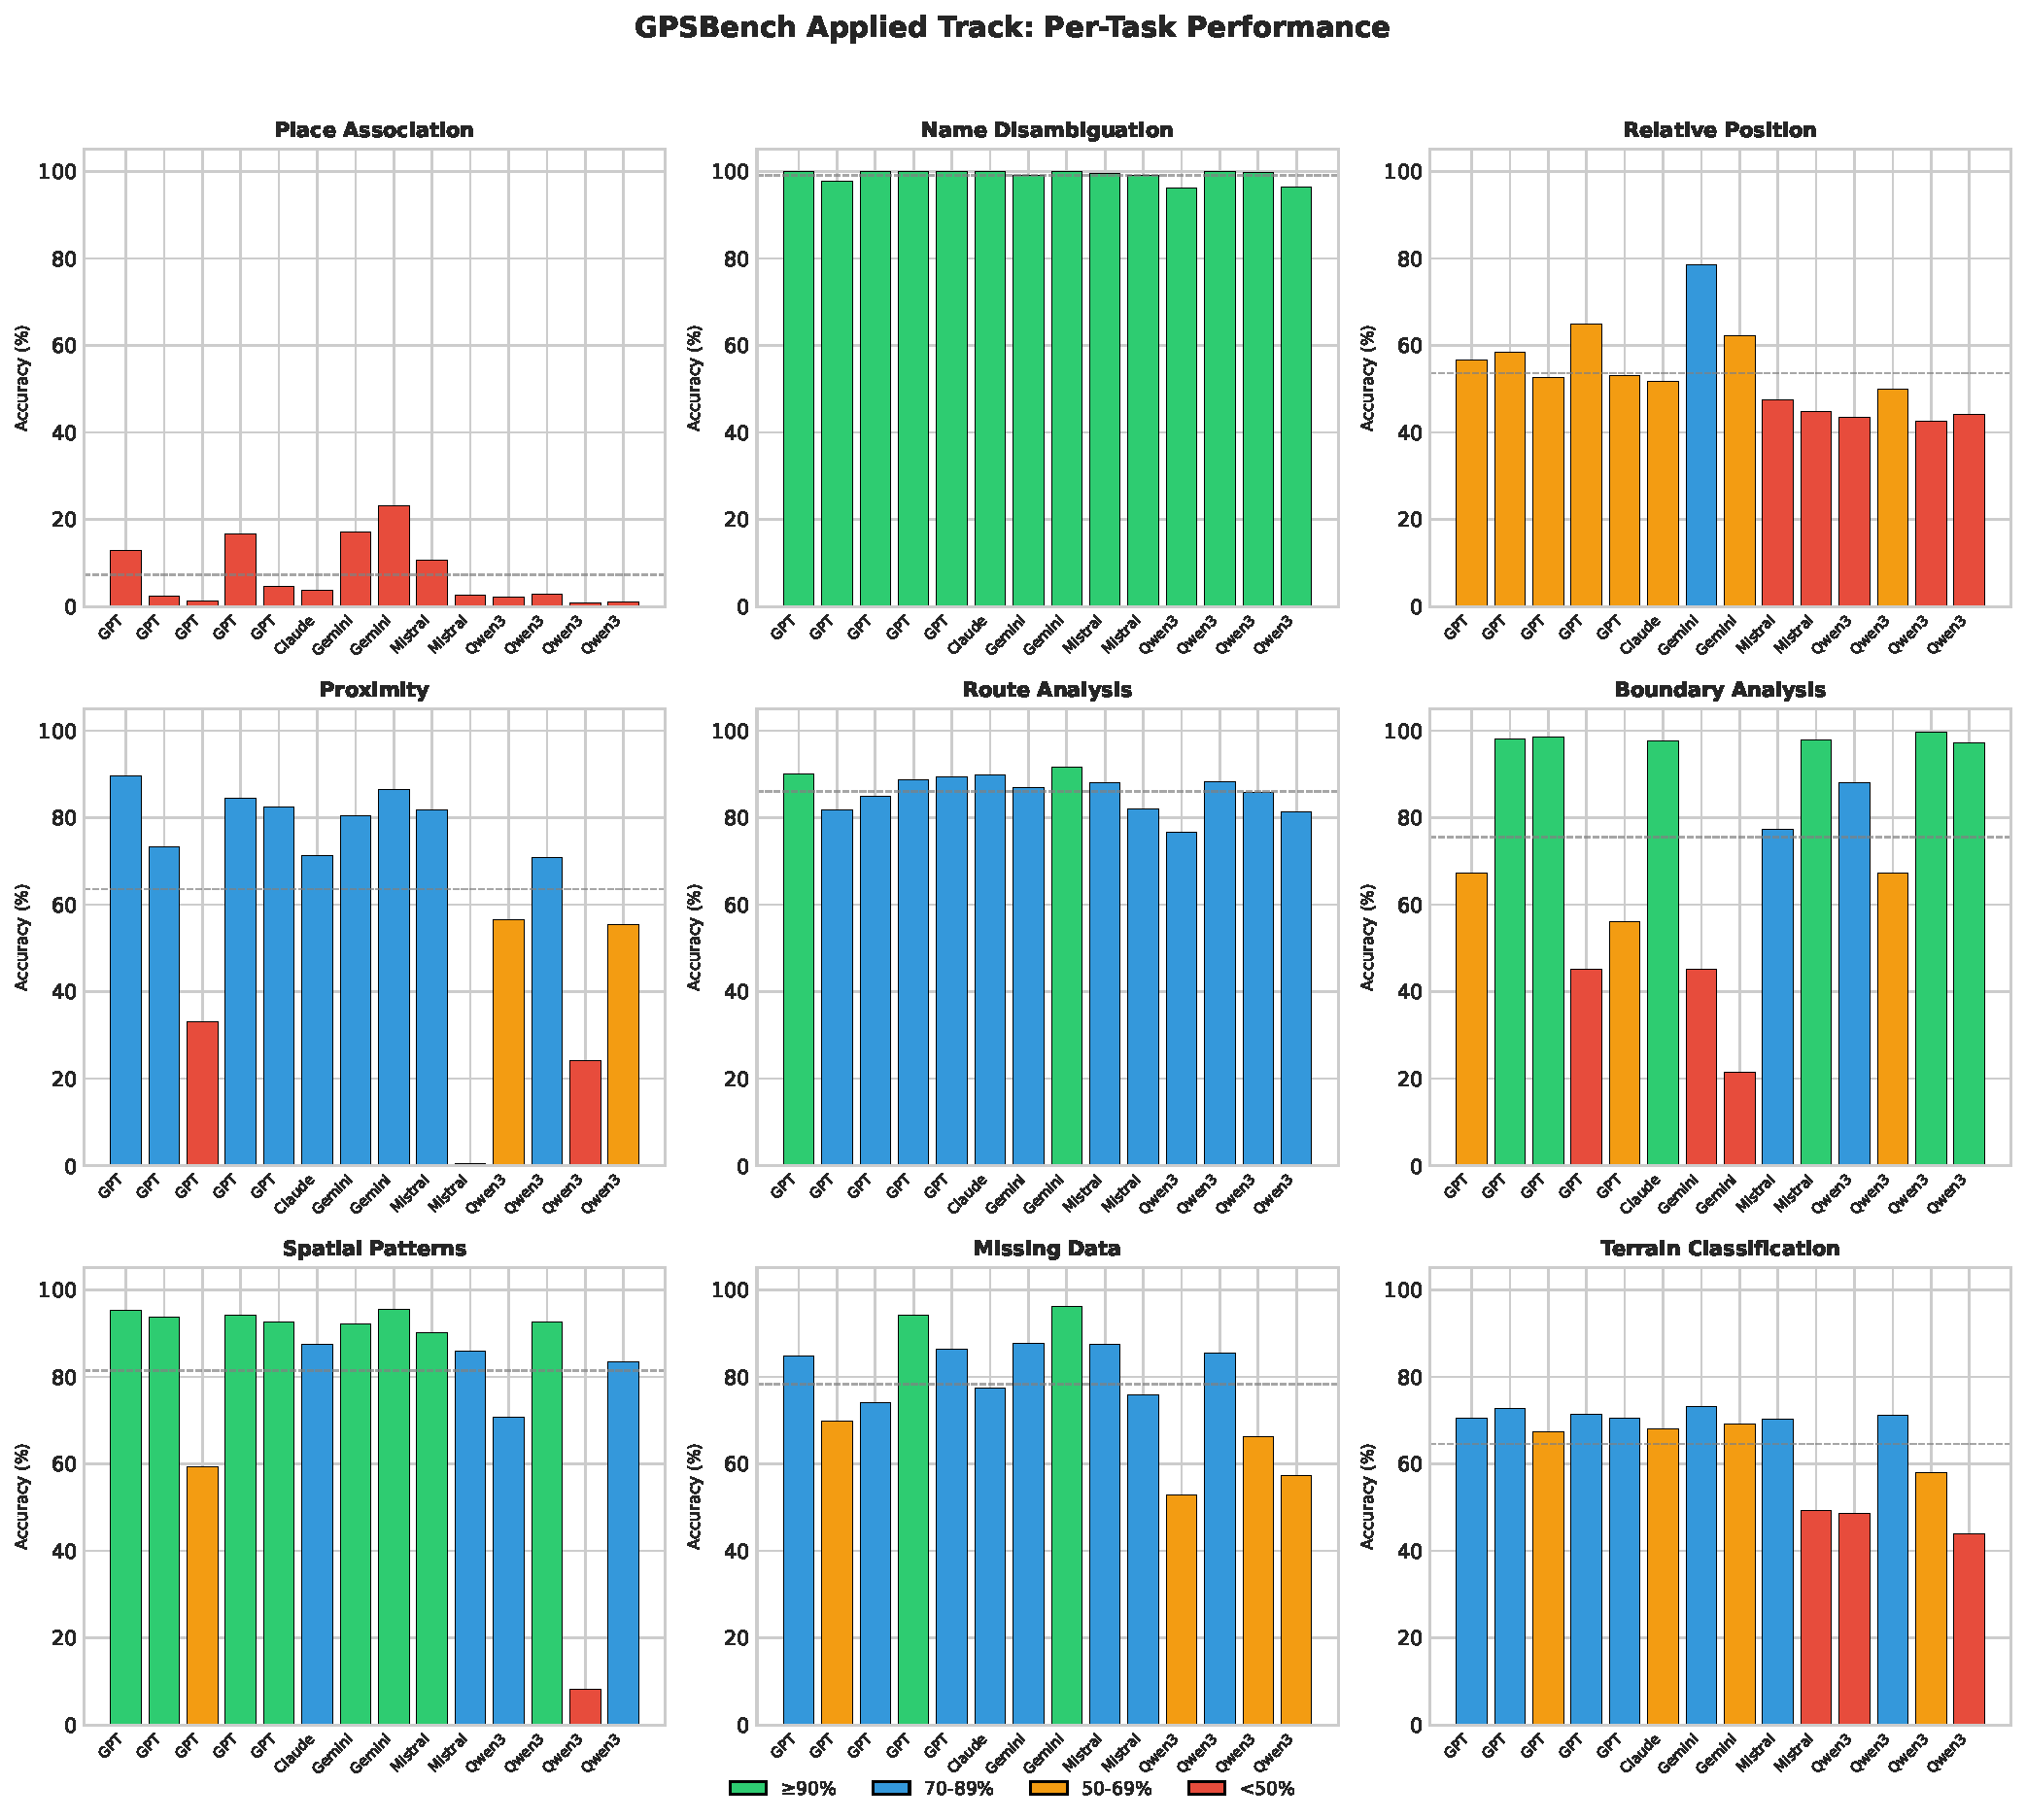
\includegraphics[width=\textwidth]{figures/per_task_applied_grid.pdf}
\caption{Per-task accuracy for the Applied Track. Color indicates performance level: green ($\geq$90\%), blue (70--89\%), orange (50--69\%), red ($<$50\%).}
\label{fig:per_task_applied}
\end{figure*}

\begin{figure*}[htbp]
\centering
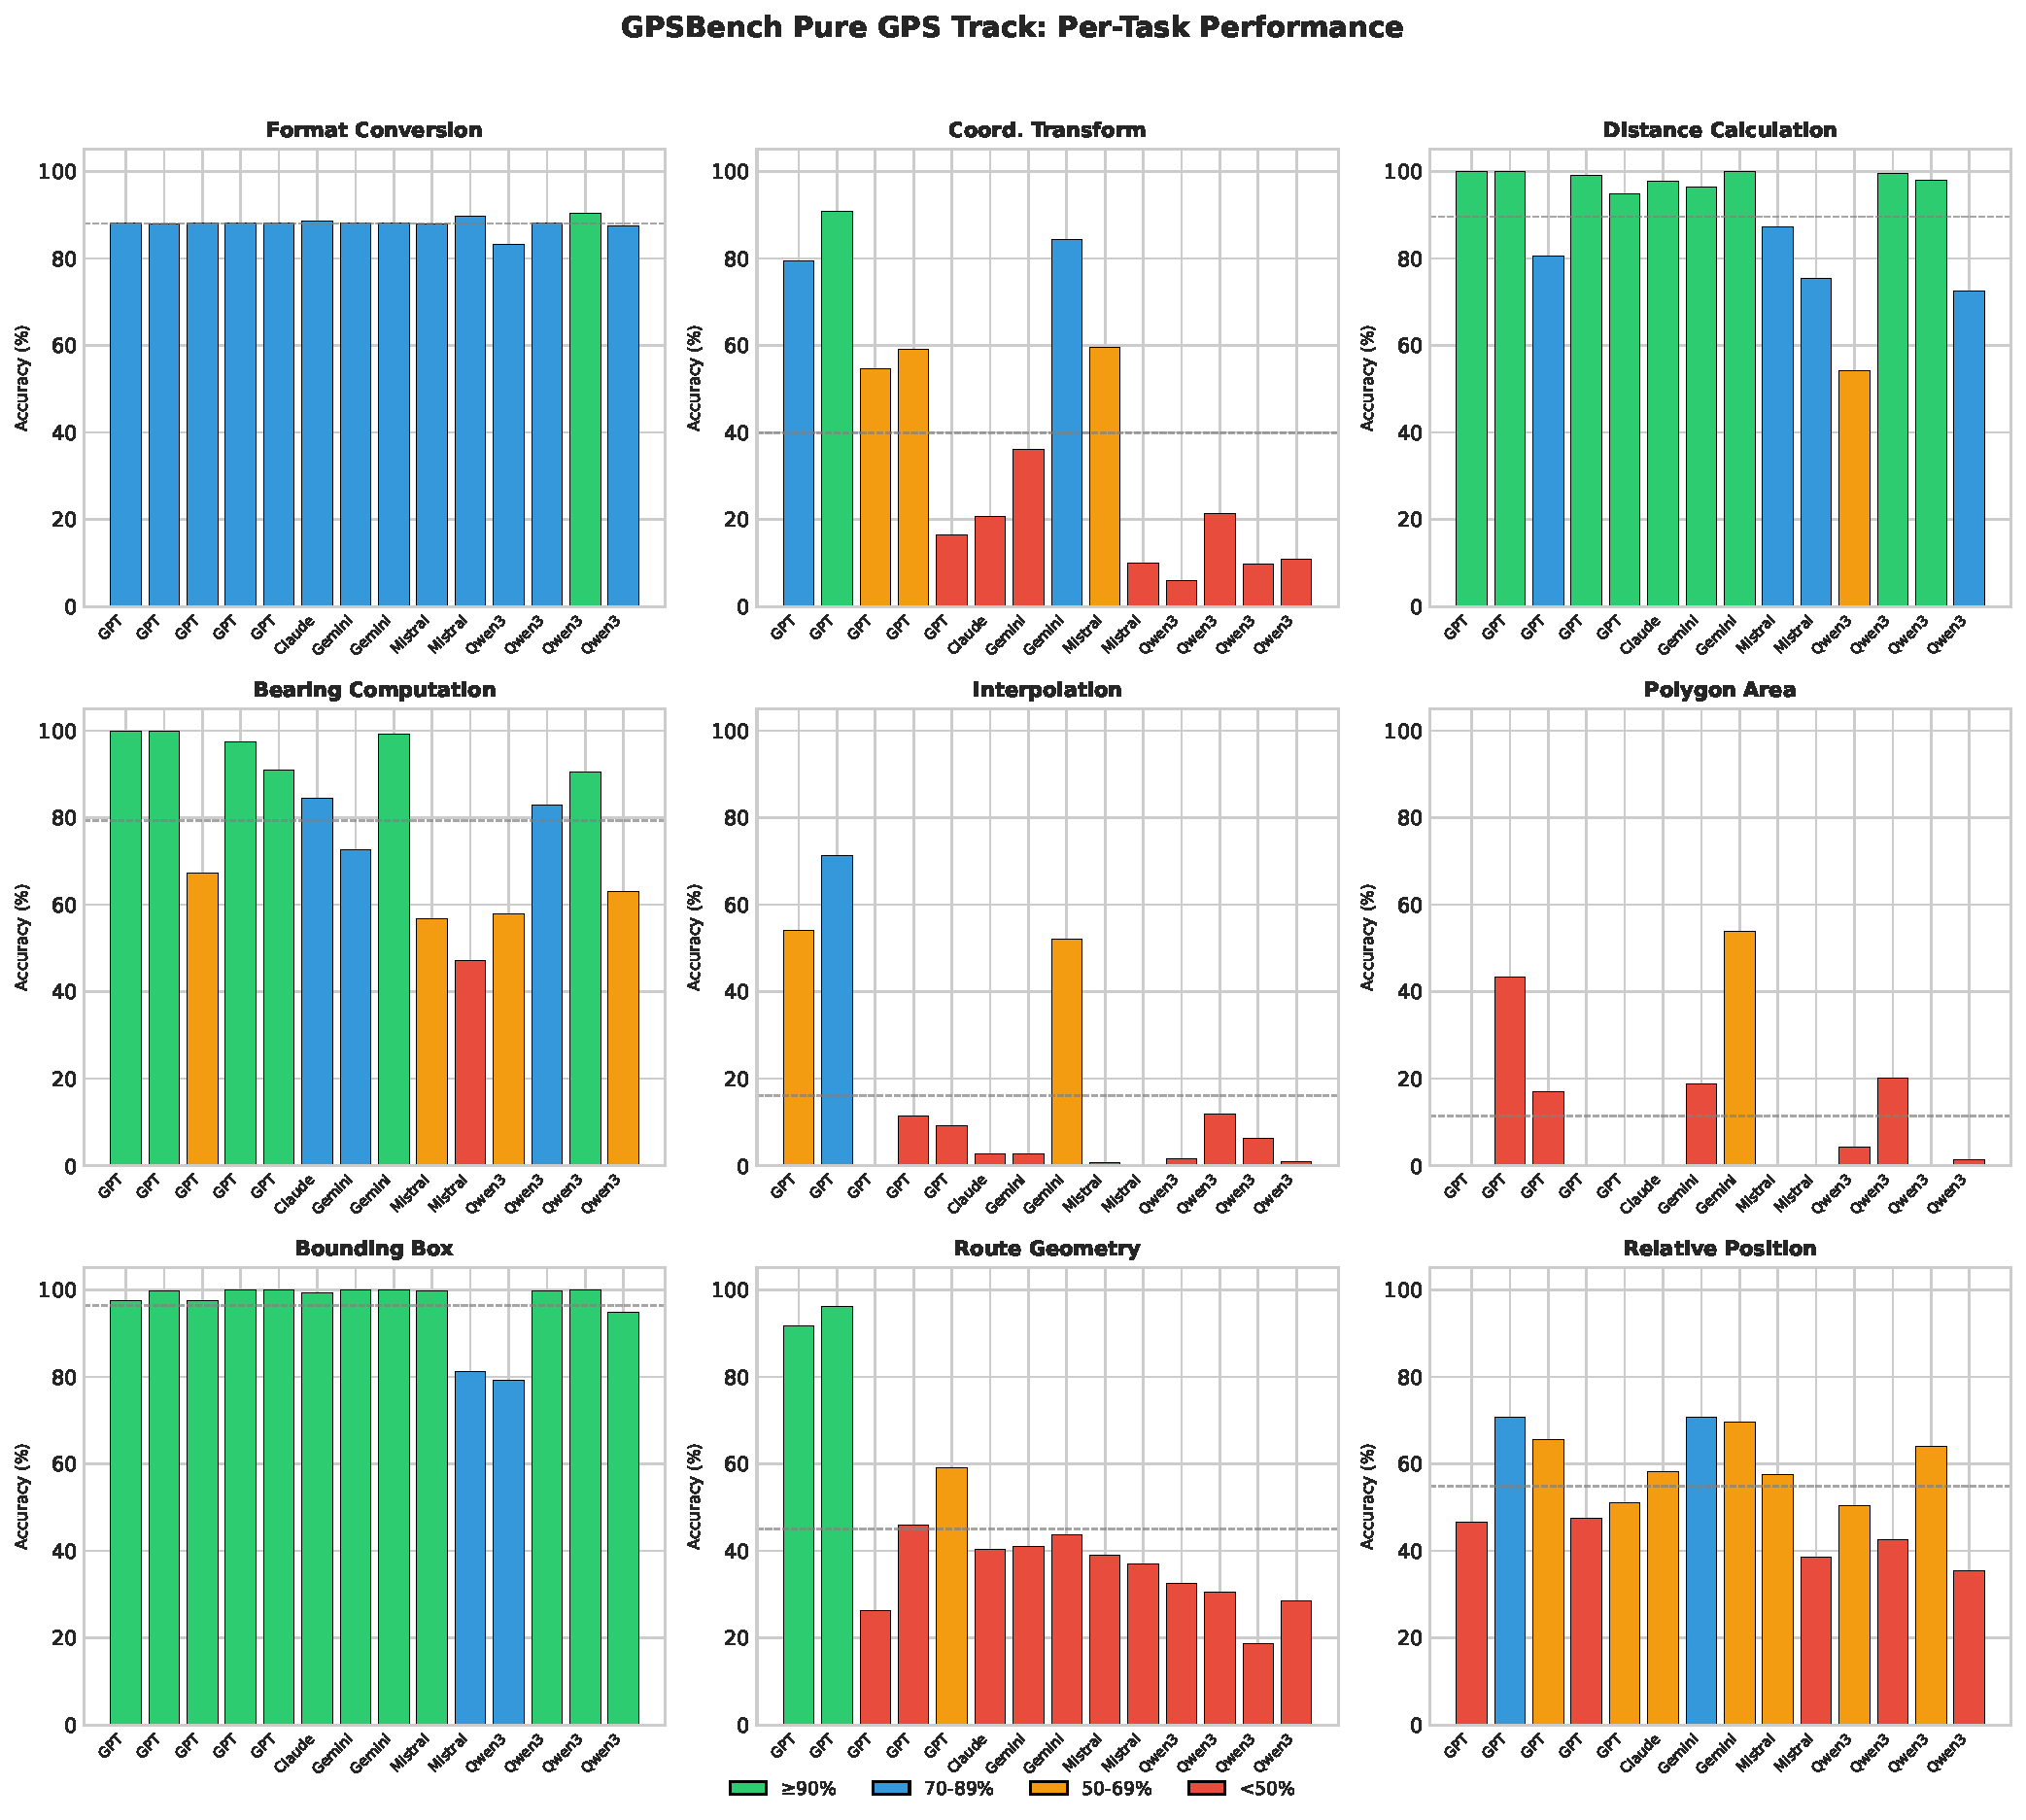
\includegraphics[width=\textwidth]{figures/per_task_pure_gps_grid.pdf}
\caption{Per-task accuracy for the Pure GPS Track. Bounding Box and Relative Position are near-solved, while Polygon Area remains unsolved across all models.}
\label{fig:per_task_pure_gps}
\end{figure*}

\paragraph{Task Difficulty Tiers.}
Tasks cluster into three distinct difficulty tiers based on mean accuracy and cross-model variance:

\begin{itemize}[leftmargin=*, itemsep=2pt]
    \item \textbf{Solved tasks} ($>$95\%, low variance): Name Disambiguation (99.2\%, std=1.2\%) and Bounding Box (96.4\%, std=6.5\%) are reliably handled by all models, indicating robust basic spatial comparison capabilities.

    \item \textbf{Brittle tasks} (50--90\%, high variance): Several tasks exhibit high variance (std$>$20\%), including Spatial Patterns (77.7\%, std=25.3\%), Bearing Computation (77.4\%, std=18.8\%), and Proximity (56.6\%, std=29.6\%). These show inconsistent performance---some models excel while others fail completely (e.g., Mistral-Small-24B scores 0.6\% on Proximity).

    \item \textbf{Unsolved tasks} ($<$20\%): Place Association (6.4\%, max=23\%), Coordinate Interpolation (15.8\%, max=71\%), and Polygon Area (11.4\%, max=54\%) are uniformly difficult. These represent fundamental capability gaps rather than model-specific limitations.
\end{itemize}

\paragraph{Applied vs.\ Pure GPS Gap.}
The mean performance gap across all 14 models is +10.0\% (std=9.7\%), indicating models generally perform better on applied reasoning than pure computation (Table~\ref{tab:track_gap}). Models with large positive gaps (Qwen3-14B: +18.5\%, Qwen3-8B: +18.3\%, Mistral-Large: +18.2\%) possess strong world knowledge but weak mathematical reasoning. Two models show negative gaps: GPT-5.1 ($-$12.4\%) and Gemini-2.5-Pro ($-$5.1\%), excelling at precise computation over contextual reasoning. Notably, GPT-5.1 achieves the highest Pure GPS accuracy (84.4\%) across all models. Note: Pure GPS scores for calculation tasks (Distance, Bearing, Area) use 1-MAPE scoring.

\begin{table}[htbp]
\centering
\caption{Performance gap between Applied and Pure GPS tracks. Positive values indicate stronger applied reasoning; negative values indicate stronger computational ability.}
\label{tab:track_gap}
\small
\begin{tabular}{lccc}
\toprule
\textbf{Model} & \textbf{Applied} & \textbf{Pure GPS} & \textbf{Gap} \\
\midrule
Qwen3-14B & 59.5 & 41.0 & +18.5 \\
Qwen3-8B & 62.2 & 43.9 & +18.3 \\
Mistral-Large & 72.5 & 54.3 & +18.2 \\
Mistral-Small-24B & 59.8 & 42.1 & +17.7 \\
Claude-Haiku-4.5 & 71.9 & 54.7 & +17.2 \\
Gemini-2.5-Flash & 73.4 & 58.5 & +14.9 \\
Qwen3-235B & 69.8 & 55.2 & +14.7 \\
GPT-4.1-mini & 70.5 & 56.6 & +13.9 \\
GPT-4.1 & 73.3 & 60.9 & +12.3 \\
GPT-5-nano & 63.5 & 55.2 & +8.2 \\
GPT-5-mini & 74.1 & 73.0 & +1.1 \\
Qwen3-30B & 53.9 & 53.1 & +0.8 \\
Gemini-2.5-Pro & 71.7 & 76.8 & $-$5.1 \\
GPT-5.1 & 72.0 & 84.4 & $-$12.4 \\
\bottomrule
\end{tabular}
\end{table}

\paragraph{Model Family Patterns.}
Aggregating by model family reveals systematic differences:
\begin{itemize}[leftmargin=*, itemsep=2pt]
    \item \textbf{GPT} (n=5): Leads on Applied tasks (70.7\%) and Pure GPS (66.0\%). GPT-5.1 achieves highest Polygon Area 1-MAPE (43\%). Gap: +4.7\%.
    \item \textbf{Gemini} (n=2): Variable performance across tracks. Gemini-2.5-Pro achieves highest Place Association (23.0\%) and strong Polygon Area (54\%). Gap: +4.9\%.
    \item \textbf{Mistral} (n=2): Largest Applied-Pure GPS gap (+17.9\%), indicating world knowledge that does not transfer to coordinate computation.
    \item \textbf{Qwen} (n=4): Including smaller dense models (8B, 14B) and larger MoE models (30B, 235B). Mean gap: +13.1\%, with smaller models showing larger gaps (+18.4\% for 8B/14B) than MoE models (+7.8\%), suggesting MoE architectures improve computational accuracy.
\end{itemize}

\paragraph{Size vs.\ Specialization.}
Large models generally outperform smaller ones. GPT-5.1 achieves the highest Pure GPS accuracy (84.4\%), outperforming GPT-5-mini (73.0\%) by 11.4\%. GPT-5.1 achieves near-perfect 1-MAPE scores on Distance (100\%) and Bearing (100\%), and leads on Area calculation (43\% 1-MAPE score vs.\ 0\% for most other models). This suggests specialized training or architectural choices can significantly impact mathematical reasoning capability.

\begin{table*}[htbp]
\centering
\caption{Per-task accuracy (\%) for Applied Track. Bold indicates best per task. Tasks ordered by mean accuracy.}
\label{tab:per_task_applied}
\small
\begin{tabular}{lccccccccc}
\toprule
\textbf{Model} & \textbf{Name} & \textbf{Route} & \textbf{Missing} & \textbf{Spatial} & \textbf{Bound.} & \textbf{Terrain} & \textbf{Prox.} & \textbf{Rel. Pos.} & \textbf{Place} \\
\midrule
GPT-5.1 & 97.7 & 81.7 & 69.9 & 93.7 & 98.1 & \textbf{72.6} & 73.3 & 58.5 & 2.5 \\
GPT-4.1 & \textbf{100.0} & 88.6 & 94.2 & 94.2 & 45.2 & 71.3 & 84.4 & 64.8 & 16.8 \\
Mistral-Large & 99.4 & 87.9 & 87.5 & 90.1 & 77.3 & 70.3 & 81.8 & 47.5 & 10.6 \\
GPT-5-mini & \textbf{100.0} & 90.1 & 84.8 & 95.2 & 67.4 & 70.6 & \textbf{89.6} & 56.6 & 12.9 \\
Claude-Haiku-4.5 & \textbf{100.0} & 89.7 & 77.5 & 87.4 & 97.6 & 68.1 & 71.3 & 51.7 & 3.6 \\
Gemini-2.5-Pro & 99.9 & \textbf{91.7} & \textbf{96.1} & \textbf{95.4} & 21.5 & 69.2 & 86.4 & 62.2 & \textbf{23.0} \\
GPT-4.1-mini & \textbf{100.0} & 89.3 & 86.3 & 92.5 & 56.0 & 70.4 & 82.4 & 53.1 & 4.7 \\
Qwen3-235B & 99.9 & 88.3 & 85.4 & 92.6 & 67.4 & 71.2 & 70.9 & 50.0 & 2.8 \\
Gemini-2.5-Flash & 99.4 & 86.9 & 87.5 & 92.1 & 47.7 & 20.7 & 80.5 & \textbf{87.2} & 17.1 \\
GPT-5-nano & 99.9 & 84.8 & 74.0 & 59.4 & 98.5 & 67.4 & 33.1 & 52.6 & 1.3 \\
Qwen3-8B & 96.4 & 81.4 & 57.4 & 83.3 & 97.2 & 43.9 & 55.5 & 44.1 & 1.0 \\
Mistral-Small-24B & 99.1 & 82.0 & 75.8 & 85.9 & 97.8 & 49.3 & 0.6 & 44.8 & 2.6 \\
Qwen3-14B & 96.2 & 76.7 & 52.9 & 70.7 & 88.0 & 48.5 & 56.5 & 43.4 & 2.2 \\
Qwen3-30B & 99.7 & 85.7 & 66.2 & 8.1 & \textbf{99.7} & 57.9 & 24.2 & 42.5 & 0.8 \\
\midrule
\textit{Mean} & \textit{99.2} & \textit{85.8} & \textit{78.5} & \textit{77.7} & \textit{77.1} & \textit{60.5} & \textit{56.6} & \textit{52.4} & \textit{6.4} \\
\textit{Std} & \textit{1.2} & \textit{4.3} & \textit{13.0} & \textit{25.3} & \textit{22.5} & \textit{14.9} & \textit{29.6} & \textit{11.2} & \textit{6.7} \\
\bottomrule
\end{tabular}
\end{table*}

\begin{table*}[htbp]
\centering
\caption{Per-task accuracy (\%) for Pure GPS Track. Bold indicates best per task. Tasks ordered by mean accuracy.}
\label{tab:per_task_pure_gps}
\small
\begin{tabular}{lccccccccc}
\toprule
\textbf{Model} & \textbf{BBox} & \textbf{Format} & \textbf{Dist.} & \textbf{Bearing} & \textbf{Rel. Pos.} & \textbf{Route} & \textbf{Coord.} & \textbf{Interp.} & \textbf{Polygon} \\
\midrule
GPT-5.1 & 99.7 & 87.8 & \textbf{99.9} & \textbf{99.9} & \textbf{70.7} & \textbf{96.3} & \textbf{90.8} & \textbf{71.4} & 43.4 \\
Gemini-2.5-Pro & \textbf{100.0} & 88.1 & \textbf{99.9} & 99.2 & 69.7 & 43.6 & 84.2 & 52.1 & \textbf{53.9} \\
GPT-5-mini & 97.5 & 88.0 & \textbf{99.9} & \textbf{99.8} & 46.6 & 91.8 & 79.4 & 54.1 & 0.0 \\
GPT-4.1 & \textbf{100.0} & 88.1 & 99.1 & 97.5 & 47.5 & 46.0 & 59.0 & 11.4 & 0.0 \\
Gemini-2.5-Flash & \textbf{100.0} & 88.0 & 96.3 & 72.7 & \textbf{70.8} & 41.0 & 36.1 & 2.7 & 18.9 \\
GPT-4.1-mini & 99.9 & 88.1 & 94.8 & 90.9 & 51.0 & 59.0 & 16.3 & 9.1 & 0.0 \\
Qwen3-235B & 99.7 & 88.1 & 99.5 & 83.0 & 42.5 & 30.5 & 21.3 & 11.9 & 20.1 \\
GPT-5-nano & 97.5 & 88.0 & 80.4 & 67.3 & 65.5 & 26.4 & 54.7 & 0.3 & 17.1 \\
Claude-Haiku-4.5 & 99.3 & 88.6 & 97.6 & 84.5 & 58.1 & 40.4 & 20.7 & 2.6 & 0.0 \\
Mistral-Large & 99.7 & 87.8 & 87.2 & 56.7 & 57.6 & 39.0 & 59.5 & 0.7 & 0.0 \\
Qwen3-30B & \textbf{100.0} & \textbf{90.4} & 97.8 & 90.5 & 64.1 & 18.7 & 9.7 & 6.4 & 0.0 \\
Mistral-Small-24B & 81.2 & 89.8 & 75.3 & 47.1 & 38.6 & 37.1 & 9.9 & 0.1 & 0.0 \\
Qwen3-8B & 94.9 & 87.5 & 72.5 & 63.0 & 35.4 & 28.5 & 10.9 & 0.9 & 1.5 \\
Qwen3-14B & 79.2 & 83.1 & 54.2 & 57.9 & 50.4 & 32.5 & 6.0 & 1.6 & 4.2 \\
\midrule
\textit{Mean} & \textit{96.4} & \textit{88.1} & \textit{89.6} & \textit{77.4} & \textit{54.6} & \textit{44.0} & \textit{39.2} & \textit{15.8} & \textit{11.4} \\
\textit{Std} & \textit{6.5} & \textit{1.8} & \textit{14.4} & \textit{18.8} & \textit{12.8} & \textit{21.9} & \textit{30.1} & \textit{24.2} & \textit{17.5} \\
\bottomrule
\end{tabular}
\end{table*}

\paragraph{Key Findings.}
\begin{enumerate}[leftmargin=*, itemsep=2pt]
    \item \textbf{High variance reveals brittle capabilities}: Several tasks have std$>$20\%, with Coord.\ Transformation (30.1\%) and Proximity (29.6\%) showing the highest variance. Models like Mistral-Small-24B score near-zero on tasks where others exceed 90\%.

    \item \textbf{Polygon Area remains unsolved}: Using 1-MAPE scoring, most models achieve 0\% (MAPE $>$100\%). Only GPT-5.1 (43\%) and Gemini-2.5-Pro (54\%) show meaningful capability, representing a fundamental gap in spherical geometry computation.

    \item \textbf{World knowledge $\neq$ computation}: The mean +10.0\% gap favoring Applied tasks, with Qwen's smaller dense models showing the largest gaps (+18.4\% for 8B/14B), demonstrates that broad language understanding does not transfer to precise coordinate manipulation.

    \item \textbf{Specialization beats scale}: GPT-5.1 achieves 84.4\% Pure GPS accuracy, surpassing all large models including GPT-5-mini (73.0\%). This 11.4\% advantage suggests architectural choices or specialized training matter more than parameter count for mathematical reasoning.
\end{enumerate}
